\chapter{Portfolio Diversification and Supporting Financial Institutions}

In Robert J. Shiller's fourth lecture on financial markets, as curated by LazyingArt LLC, the mathematics is introduced only after the institutional world is in place. We begin with the VOC, the Amsterdam exchange, brokers, street-name ownership, short sales, and limited liability. Only then do we ask the lecture's central quantitative question: if expected returns, variances, and covariances are given, what is the right way to think about a portfolio? The answer comes in stages: leverage, hyperbolas, diversification, tangency, and finally the idea that the risk which matters in equilibrium is covariance with the market.

\section{Finance as Institutional Invention}

The lecture opens by carrying forward a theme from the previous class: finance is not merely a list of contracts, but a kind of engineering. Financial devices are invented, experimented with, discarded when they fail, and copied around the world when they work. The historical bridge for this lecture is the Verenigde Oostindische Compagnie, founded in 1602, together with the Amsterdam Stock Exchange created to trade its shares.

\begin{definition}
A portfolio is a collection of investments held over a specified horizon.
\end{definition}

This historical prelude matters because the lecture does not want to treat portfolio theory as an abstract optimization exercise detached from institutions. The VOC was a long-lived venture, unlike the older one-voyage merchant partnerships that dissolved after a single trip. Once we have a durable company with tradable shares, a series of further institutions appears almost automatically.

First, shares become tradable every day rather than only when the company reopens its books. Second, brokers hold inventories of shares and mediate transactions. Third, ownership is effectively held in street name: the broker's books tell the investor that he owns the shares even before the company itself has updated its own records. Once that arrangement exists, a broker can sell more shares than he currently owns and promise to obtain them later. In modern language, short interest emerges endogenously from the trading mechanism itself.

The lecture emphasizes that this is not a historical curiosity. It is a general lesson. Once a large, long-lived, democratic company is created and once its shares are tradable through intermediaries, speculation, disagreement, and volatility arise naturally. Some traders become enthusiastic buyers; others, like the Dutch short seller discussed in the lecture, become aggressive pessimists. The market becomes liquid because the asset is uncertain, and uncertain because it is liquid.

Limited liability is equally important. If shareholders can lose no more than the funds they invest, then a much wider public can participate in risky enterprise. We can speculate on global trade without risking personal ruin beyond the amount already committed. In that sense the stock market is a social technology: it channels gambling instincts into the financing of ships, trading posts, and durable enterprise.

This is the setting from which the rest of the lecture emerges. Portfolio theory is not introduced as a detached theorem. It is introduced because once tradable risky assets exist, we must ask how to live with them.

\section{The Equity Premium Puzzle}

The first major conceptual turn in the lecture is the equity premium puzzle. The VOC story supplies the intuition. If a stock appears to earn extraordinary returns for long stretches, why does capital not rush in until the exceptional advantage disappears?

The lecture then broadens the question beyond the VOC and points to long-run evidence. For the United States, the reported real geometric average return on stocks is about \(6.8\%\) per year, while the real return on short-term government securities is about \(2.8\%\). So the long-run gap is roughly
\begin{equation}
6.8\% - 2.8\% = 4.0\%.
\end{equation}
International evidence points in the same direction. Across the countries discussed in the lecture, the equity premium is not uniquely American; it appears in many national markets, with magnitudes on the order of \(3\%\) to \(6\%\).

The puzzle is not that stocks sometimes outperform. The puzzle is that they seem, over very long stretches, to outperform safer assets persistently enough that one is tempted to ask why everyone does not simply hold stocks.

\subsection{Question \& Answer}

\paragraph{Question.} If stocks do so well, why does everyone not simply hold them?

\paragraph{Answer.} The lecture's provisional answer is risk, but only provisionally. It is not enough to say vaguely that stocks fluctuate more. That answer is too loose, and the remainder of the lecture is devoted to sharpening it. We need a theory that distinguishes between a high-return asset and a well-chosen portfolio, and we need a definition of risk that survives diversification rather than disappearing under it.

This is the point at which the lecture introduces Harry Markowitz. Before 1952, investors already knew the proverb about not putting all their eggs in one basket. But the lecture insists that this was not yet a theory. It was advice without an optimization problem. Markowitz's contribution was to ask, in a mathematically definite way: if we know expected returns, variances, and covariances, what portfolio should we choose?

\section{Markowitz's Breakthrough and the One-Risky-One-Riskless Case}

The lecture is careful about what makes Markowitz a breakthrough. He did not merely say that diversification is prudent. He asked for the best portfolio given a collection of statistics. That sounds obvious only after the fact. In the lecture's telling, this is precisely what is astonishing: sophisticated financial systems existed for centuries before anyone posed portfolio choice in that clean mathematical form.

The lecture begins the mathematics with the simplest nontrivial case. There is one risky asset and one riskless asset. The risky asset may be imagined first as the VOC itself; the riskless asset may be imagined as a short government claim whose maturity matches the investor's horizon.

\subsection{Question \& Answer}

\paragraph{Question.} If leverage lets us reach many target returns from one risky asset, what could an ``optimal portfolio'' even mean?

\paragraph{Answer.} It cannot mean ``the best asset'' in isolation. Once borrowing, lending, and shorting are allowed, one risky asset already generates an entire family of feasible portfolios. What matters is not a best investment in the crude sense, but a tradeoff between expected return and risk. That shift in viewpoint is the first essential Markowitz lesson.

\begin{figure}[h]
\centering

\includegraphics[width=0.82\textwidth]{lecture_04_figure_02.png}
\caption{Lecture slide: risky and riskless asset portfolio formulas.}
\end{figure}

The slide shown in the lecture uses the phrase ``portfolio expected value,'' but the content is clearly the expected return on the portfolio. We standardize the notation slightly while preserving the lecture's order of steps. If we place a fraction \(x\) of wealth in the risky asset and \(1-x\) in the riskless asset, then
\begin{align}
r_p &= x r_1 + (1-x)r_f, \\
\operatorname{Var}(r_p) &= x^2 \operatorname{Var}(r_1), \\
\sigma_p &= |x| \sigma_1.
\end{align}
The second line uses the fact that the riskless return is known at the horizon. The lecture then solves for \(x\) in terms of the target expected return:
\begin{equation}
x = \frac{r_p-r_f}{r_1-r_f}.
\end{equation}
Substituting this into the standard-deviation expression gives
\begin{equation}
\sigma_p
=
\left|
\frac{r_p-r_f}{r_1-r_f}
\right|
\sigma_1.
\end{equation}

\paragraph{Worked example.}
The lecture's numerical example fixes the riskless rate at \(5\%\), the risky asset's expected return at \(20\%\), and the risky asset's standard deviation at \(40\%\).

\begin{enumerate}
\item If we invest our own \(100\) guilders entirely in the risky asset, the expected profit is \(20\) guilders and the standard deviation is \(40\) guilders.
\item If we borrow another \(100\) guilders and invest \(200\) guilders in the risky asset, then the expected gain on the asset side is \(40\) guilders, but we owe \(5\) guilders in interest. So the expected return on our original wealth is
\begin{equation}
2(20\%) - 5\% = 35\%.
\end{equation}
The standard deviation scales with the position size:
\begin{equation}
2(40\%) = 80\%.
\end{equation}
\item If instead we short \(200\) guilders of the risky asset, we expect to lose \(40\) guilders on that short position, while the \(300\) guilders held in cash earn \(5\%\). The expected return on our original wealth is then
\begin{equation}
-2(20\%) + 3(5\%) = -25\%.
\end{equation}
\end{enumerate}

The geometric conclusion is immediate. In \((\sigma_p, E[r_p])\)-space, the feasible set is a broken straight line issuing from the riskless point: one branch for lending and leveraged long positions, the other for short positions. The lecture explicitly calls this a degenerate case of a hyperbola.

\begin{figure}[h]
\centering
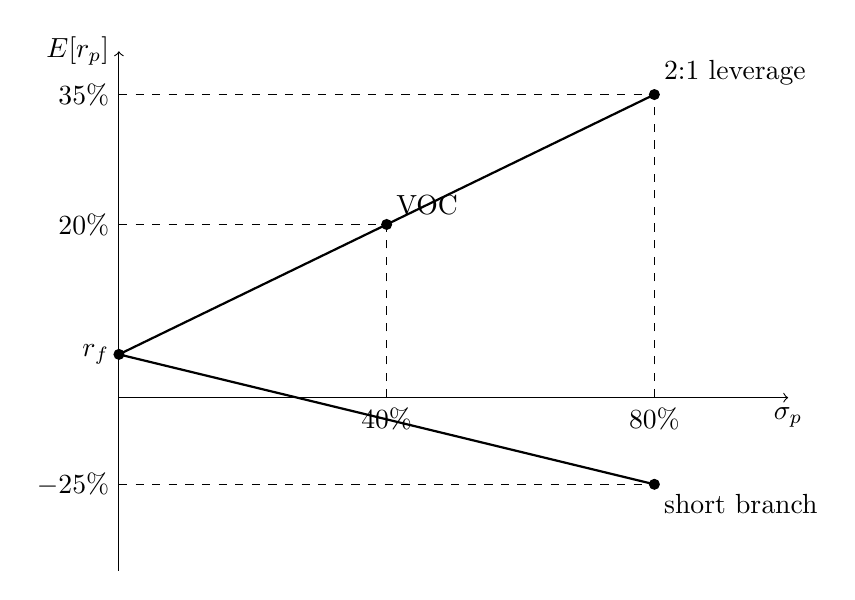
\begin{tikzpicture}[x=0.85cm,y=0.55cm]
\draw[->] (0,0) -- (10,0) node[below] {$\sigma_p$};
\draw[->] (0,-4) -- (0,8) node[left] {$E[r_p]$};

\draw[thick] (0,1) -- (8,7);
\draw[thick] (0,1) -- (8,-2);

\fill (0,1) circle (2pt);
\fill (4,4) circle (2pt);
\fill (8,7) circle (2pt);
\fill (8,-2) circle (2pt);

\draw[dashed] (4,0) -- (4,4);
\draw[dashed] (0,4) -- (4,4);
\draw[dashed] (8,0) -- (8,7);
\draw[dashed] (0,7) -- (8,7);
\draw[dashed] (0,-2) -- (8,-2);

\node[left] at (0,1) {$r_f$};
\node[above right] at (4,4) {VOC};
\node[above right] at (8,7) {2:1 leverage};
\node[below right] at (8,-2) {short branch};
\node[below] at (4,0) {$40\%$};
\node[below] at (8,0) {$80\%$};
\node[left] at (0,4) {$20\%$};
\node[left] at (0,7) {$35\%$};
\node[left] at (0,-2) {$-25\%$};
\end{tikzpicture}
\caption{Transcript-based reconstruction of the one-risky-one-riskless opportunity set.}
\end{figure}

The point is not that one point on this broken line is universally best. The point is that the client can ask for any target return, and we can often produce it simply by changing leverage. The naive language of ``best investment'' has already broken down.

\section{Two Risky Assets and the Efficient Frontier}

Only now do we arrive at the first genuine Markowitz geometry. The lecture temporarily sets the riskless asset aside and asks us to consider two risky assets. In the concrete example, these are U.S. stocks and long-term Treasury bonds held over a one-year horizon. The latter are called ``bonds'' in the lecture, but they are not riskless here, because their market price fluctuates over the year.

\begin{figure}[h]
\centering

\includegraphics[width=0.82\textwidth]{lecture_04_figure_03.png}
\caption{Lecture slide: two-asset frontier variance substitution.}
\end{figure}

If \(x_1\) is the weight in asset \(1\) and \(1-x_1\) is the weight in asset \(2\), then
\begin{equation}
r_p = x_1 r_1 + (1-x_1)r_2.
\end{equation}
Solving this for \(x_1\) gives the substitution displayed in the lecture:
\begin{equation}
x_1 = \frac{r_p-r_2}{r_1-r_2}.
\end{equation}
The two-asset variance formula is
\begin{equation}
\sigma_p^2 = x_1^2 \sigma_1^2 + (1-x_1)^2 \sigma_2^2 + 2x_1(1-x_1)\sigma_{12}.
\end{equation}
Substituting for \(x_1\), we obtain the frontier as a relation between standard deviation and expected return:
\begin{align}
\sigma_p^2
&=
\left(
\frac{r_p-r_2}{r_1-r_2}
\right)^2
\sigma_1^2
+
\left(
\frac{r_1-r_p}{r_1-r_2}
\right)^2
\sigma_2^2
+
2
\frac{(r_p-r_2)(r_1-r_p)}{(r_1-r_2)^2}
\sigma_{12}.
\end{align}

This is the first real hyperbola of the lecture. The covariance term \(\sigma_{12}\) is the essential new ingredient. If two assets do not move perfectly together, their combination can bend inward in risk-return space. Diversification is no longer a proverb; it becomes a piece of geometry.

\begin{figure}[h]
\centering
\begin{tikzpicture}[x=0.48cm,y=0.55cm]
\draw[->] (0,0) -- (22,0) node[below] {$\sigma_p$};
\draw[->] (0,0) -- (0,10) node[left] {$E[r_p]$};

\draw[thick] plot[smooth] coordinates {(7.0,5.4) (8.0,6.1) (10.0,6.9) (13.5,7.9) (18.0,8.8)};
\draw[thick,dashed] plot[smooth] coordinates {(7.0,5.4) (7.8,4.8) (9.5,4.0) (12.5,2.6)};

\fill (9.5,4.0) circle (2pt);
\fill (8.2,5.8) circle (2pt);
\fill (10.2,6.6) circle (2pt);
\fill (16.0,8.3) circle (2pt);

\node[below] at (9.5,4.0) {100\% bonds};
\node[left] at (8.2,5.8) {$25/75$};
\node[above] at (10.2,6.6) {$50/50$};
\node[right] at (16.0,8.3) {100\% stocks};

\draw[dotted] (7.0,0) -- (7.0,5.4);
\node[below] at (7.0,0) {$\sigma_{\min}$};
\node[above right] at (13.2,7.8) {efficient frontier};
\end{tikzpicture}
\caption{Simplified redraw of the two-asset opportunity set. The efficient frontier is the upper branch above the minimum-variance point.}
\end{figure}

The lecture's first sharp investment conclusion appears here. A \(100\%\) bond portfolio is not merely conservative. It is dominated. There exists a stock-bond mixture with the same standard deviation and a higher expected return. So the efficient frontier is not the whole hyperbola. It is only the upper branch above the minimum-variance point.

That is why the lecture insists on a distinction between feasible and efficient. Many portfolios are possible. Fewer are worth choosing.

\section{Three Assets, Diversification, and Oil}

The lecture then adds a third risky asset: oil. The qualitative claim is that oil is important, pays a good return, and is not highly correlated with the stock market. The result is a frontier that shifts leftward: for a given expected return, the investor can attain lower standard deviation.

\begin{remark}
At this point the transcript garbles some subscripts in the three-asset formulas. The standard completion below matches the lecture's intention and the visible frontier geometry. It should be read as a cautious normalization rather than a verbatim transcription of every spoken symbol.
\end{remark}

With three risky assets, the expected return remains a weighted average:
\begin{equation}
r_p = x_1 r_1 + x_2 r_2 + x_3 r_3,
\qquad
x_1+x_2+x_3=1.
\end{equation}
The portfolio variance is
\begin{align}
\sigma_p^2
&=
x_1^2 \sigma_1^2
+
x_2^2 \sigma_2^2
+
x_3^2 \sigma_3^2
+
2x_1x_2 \sigma_{12}
+
2x_1x_3 \sigma_{13}
+
2x_2x_3 \sigma_{23}.
\end{align}
For any target \(r_p\), we may ask for the minimum-variance mixture satisfying these constraints. The lecture's chart is exactly a picture of that optimization.

\begin{figure}[h]
\centering

\includegraphics[width=0.88\textwidth]{lecture_04_figure_04.png}
\caption{Lecture slide: efficient frontier with and without oil.}
\end{figure}

The original stock-bond frontier remains on the slide as the weaker comparison set, labeled ``W/O Oil.'' Once oil is added, the relevant opportunity set becomes the left-shifted frontier. In the visible labels we can read sample portfolios such as \(100\%\) bonds, \(50\%\) stocks and \(50\%\) bonds, \(100\%\) stocks, and mixtures such as \(15\%\) oil, \(53\%\) stocks, \(32\%\) bonds, or \(21\%\) oil, \(79\%\) stocks, \(0\%\) bonds. One of the upper labels even uses a negative bond weight, showing that the frontier can accommodate leverage as well as diversification.

\begin{figure}[h]
\centering
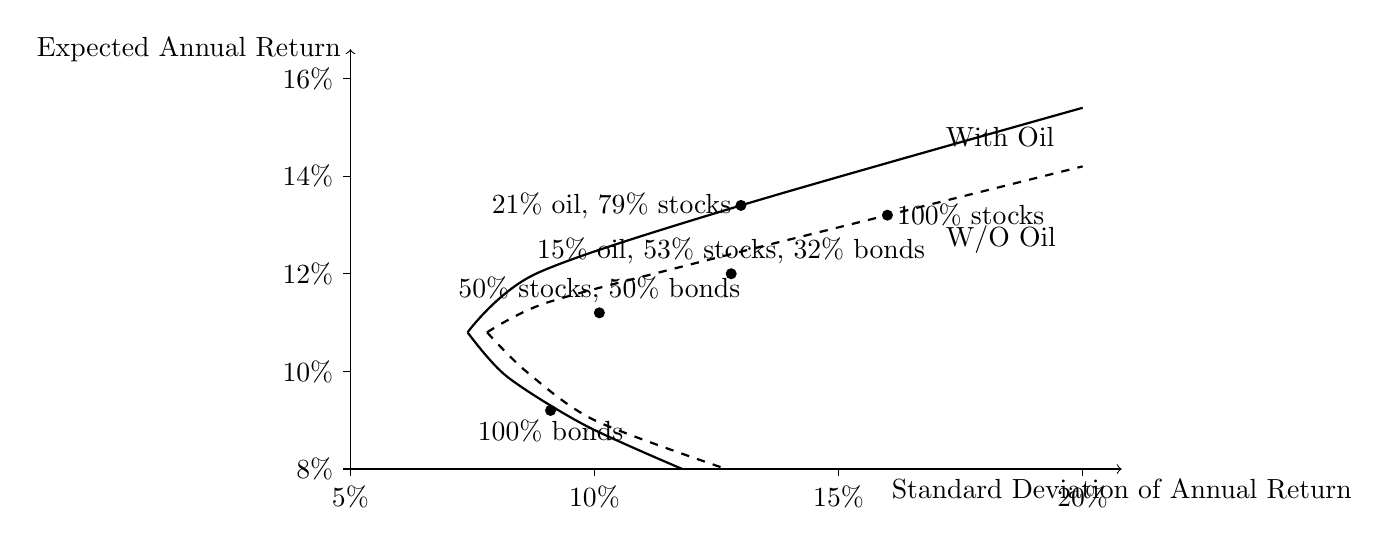
\begin{tikzpicture}[x=0.62cm,y=0.62cm]
\draw[->] (5,8) -- (20.8,8) node[below] {Standard Deviation of Annual Return};
\draw[->] (5,8) -- (5,16.6) node[left] {Expected Annual Return};

\foreach \x in {5,10,15,20}
{
  \draw (\x,8) -- (\x,7.85);
  \node[below] at (\x,7.85) {\(\x\%\)};
}
\foreach \y in {8,10,12,14,16}
{
  \draw (5,\y) -- (4.85,\y);
  \node[left] at (4.85,\y) {\(\y\%\)};
}

\draw[thick,dashed] plot[smooth] coordinates {(7.8,10.8) (9.0,11.4) (12.0,12.2) (16.0,13.2) (20.0,14.2)};
\draw[thick,dashed] plot[smooth] coordinates {(7.8,10.8) (8.6,10.0) (10.0,9.0) (12.7,8.0)};

\draw[thick] plot[smooth] coordinates {(7.4,10.8) (8.8,12.0) (13.0,13.4) (20.0,15.4)};
\draw[thick] plot[smooth] coordinates {(7.4,10.8) (8.2,9.9) (9.8,8.9) (11.8,8.0)};

\fill (9.1,9.2) circle (2pt);
\fill (10.1,11.2) circle (2pt);
\fill (12.8,12.0) circle (2pt);
\fill (16.0,13.2) circle (2pt);
\fill (13.0,13.4) circle (2pt);

\node[below] at (9.1,9.2) {100\% bonds};
\node[above] at (10.1,11.2) {50\% stocks, 50\% bonds};
\node[above] at (12.8,12.0) {\(15\%\) oil, \(53\%\) stocks, \(32\%\) bonds};
\node[right] at (16.0,13.2) {100\% stocks};
\node[left] at (13.0,13.4) {\(21\%\) oil, \(79\%\) stocks};

\node[right] at (17.0,14.8) {With Oil};
\node[right] at (17.0,12.7) {W/O Oil};
\end{tikzpicture}
\caption{Simplified redraw of the frontier comparison, preserving the lecture's truncated horizontal axis beginning at \(5\%\).}
\end{figure}

The lecture interprets the leftward shift in very plain terms: the more different kinds of assets we can put into the portfolio, the lower we can make the standard deviation for a given expected return. That is the mathematical content of diversification.

The lecture then turns from geometry back to institutions. Norway, rich in North Sea oil, is described as holding far too much implicit oil exposure relative to the frontier. A portfolio like \(15\%\) oil, \(53\%\) stocks, \(32\%\) bonds would be far better diversified than effectively holding \(100\%\) oil. Yet politics intervenes. Governments hesitate to hedge what they regard as national patrimony. The lecturer's proposed remedy is not necessarily to sell the oil outright, but to reduce exposure through derivative transactions, such as shorting oil futures. The obstacle is not arithmetic; it is politics.

Mexico appears as a similar case. The point is not that public officials are irrational. It is that institutional and political constraints can keep actual portfolios away from mathematically efficient ones. The lecture thus returns to its opening theme: theory lives inside institutions.

\begin{figure}[h]
\centering

\includegraphics[width=0.88\textwidth]{lecture_04_figure_05.png}
\caption{Lecture slide: the horizontal axis begins at \(5\%\), not at zero.}
\end{figure}

This second screenshot of the oil chart matters because the lecturer points directly to the left end of the horizontal axis and notes that the slide does not show zero. That omission becomes important in the next step. Once the riskless asset is brought back, the relevant line starts at zero standard deviation, not at \(5\%\) standard deviation. The chart is a convenient visual summary of risky portfolios, but it is not the whole geometry yet.

\section{The Riskless Asset Returns: Tangency, Mutual Funds, and Market Risk}

Now the lecture adds the riskless asset back into the many-asset world. We should think of the riskless claim as a one-year government security whose maturity matches the investor's one-year horizon. Its return is therefore known at the horizon, so it sits at zero standard deviation.

Take any efficient risky portfolio on the frontier. If we mix it with the riskless asset, we obtain a straight line in mean-standard-deviation space. The lecture's idea is to draw all such lines through the riskless point and then ask which one lies highest. The answer is the line that is tangent to the efficient risky frontier. Its point of tangency is the tangency portfolio.

If \(r_T\) and \(\sigma_T\) denote the expected return and standard deviation of that tangency portfolio, then every mixture of the riskless asset and the tangency portfolio lies on the capital market line
\begin{equation}
E[r_p] = r_f + \frac{E[r_T]-r_f}{\sigma_T}\,\sigma_p.
\end{equation}
This is not presented in the lecture as a full formal derivation, but it is the standard equation corresponding to the geometry Shiller describes.

The lecture's practical point is decisive. Once the riskless asset is available, many risky frontier portfolios become dominated. A portfolio such as \(15\%\) oil, \(53\%\) stocks, \(32\%\) bonds may have been efficient within the set of risky portfolios alone, but it can be beaten by taking an appropriate mixture of the tangency portfolio and the riskless asset. So the addition of the riskless asset collapses the relevant choice set to a single risky fund plus a borrowing or lending decision.

\begin{proposition}
Under the lecture's Markowitz assumptions---shared expected returns, shared variances and covariances, and the ability to borrow or lend at the riskless rate---every efficient portfolio is a mixture of the riskless asset and the same tangency portfolio.
\end{proposition}

\begin{proof}
Any efficient portfolio using the riskless asset must lie on a straight line joining the riskless point to some risky portfolio on the efficient frontier. Among all such lines, only the one with maximal slope delivers the highest expected return for each attainable standard deviation. That maximal-slope line is tangent to the risky frontier. Hence every efficient investor chooses a point on that same line and therefore differs from every other efficient investor only in the fraction allocated to the riskless asset versus the tangency portfolio.
\end{proof}

This is the mutual fund theorem in the lecture's form. One does not need thousands of fundamentally different efficient risky funds. One needs one risky fund---the tangency portfolio---and then different investors lever or de-lever it according to taste.

The lecture then pushes one step further. If everyone wants to hold the same risky portfolio, then in equilibrium that portfolio must coincide with the aggregate portfolio of risky assets outstanding. Supply must match demand. Thus
\begin{equation}
\text{market portfolio} = \text{tangency portfolio}.
\end{equation}

This is the bridge from Markowitz geometry to the capital asset pricing model. The lecture does not pretend to derive CAPM in full. It states the standard relation and then explains its meaning:
\begin{equation}
E[r_i] = r_f + \beta_i\bigl(E[r_M]-r_f\bigr),
\end{equation}
where
\begin{equation}
\beta_i = \frac{\operatorname{Cov}(r_i,r_M)}{\operatorname{Var}(r_M)}.
\end{equation}
The crucial interpretive claim is that investors do not care about the standalone variance of a small asset once it is placed inside a large diversified portfolio. Independent fluctuations can be averaged away. What remains costly is covariance with the market, because that is the risk that cannot be diversified out.

In the lecture's language, we must change our idea of what risk is. Risk is not mere uncertainty. Risk, in equilibrium, is co-movement with the market. A high-beta asset is one that moves more strongly with the general market and therefore must offer a higher expected return.

The lecture gives Apple as an example of a stock with beta greater than one, roughly \(1.5\). That does not mean merely that Apple is volatile. It means that Apple moves with the market in an amplified way. That market exposure, not variance in isolation, is what commands a premium.

The final practical coda is the Sharpe ratio. For any portfolio,
\begin{equation}
S_p = \frac{E[r_p]-r_f}{\sigma_p}.
\end{equation}
Along the capital market line this ratio is constant, because it is simply the slope of the line from the riskless point to the portfolio. That is why the Sharpe ratio becomes a leverage-adjusted measure of performance. A manager who advertises a high average return may simply be levering an ordinary risky strategy. The Sharpe ratio asks how much excess return was produced per unit of total standard deviation.

This is the lecture's closing moral. The theory does not only classify portfolios. It teaches us how to evaluate portfolio managers. We do not ask first for raw return. We ask what risk and what leverage produced it.

\section{Summary}

The lecture begins with institutions and ends with equilibrium asset pricing. The path matters. A stock market first appears as a social invention: the VOC, brokers, street-name ownership, short interest, limited liability, and volatile trade. That institutional world then raises the equity-premium puzzle. Markowitz enters by turning vague advice about diversification into a mathematically definite problem. With one risky asset and one riskless asset, we learn that there is no single best investment, only a tradeoff. With two and then three risky assets, the geometry becomes hyperbolic and diversification becomes visible. With the riskless asset added back, the tangency portfolio emerges, the mutual fund theorem follows, and the market portfolio becomes the equilibrium risky fund. CAPM then sharpens the intuition: the risk that matters is covariance with the market, while the Sharpe ratio gives the practical measure of performance once leverage is taken seriously.